% \chapter{Fractures}
% \chapter{Introduction}
\begin{figure}[htpb]%
    \centering%
    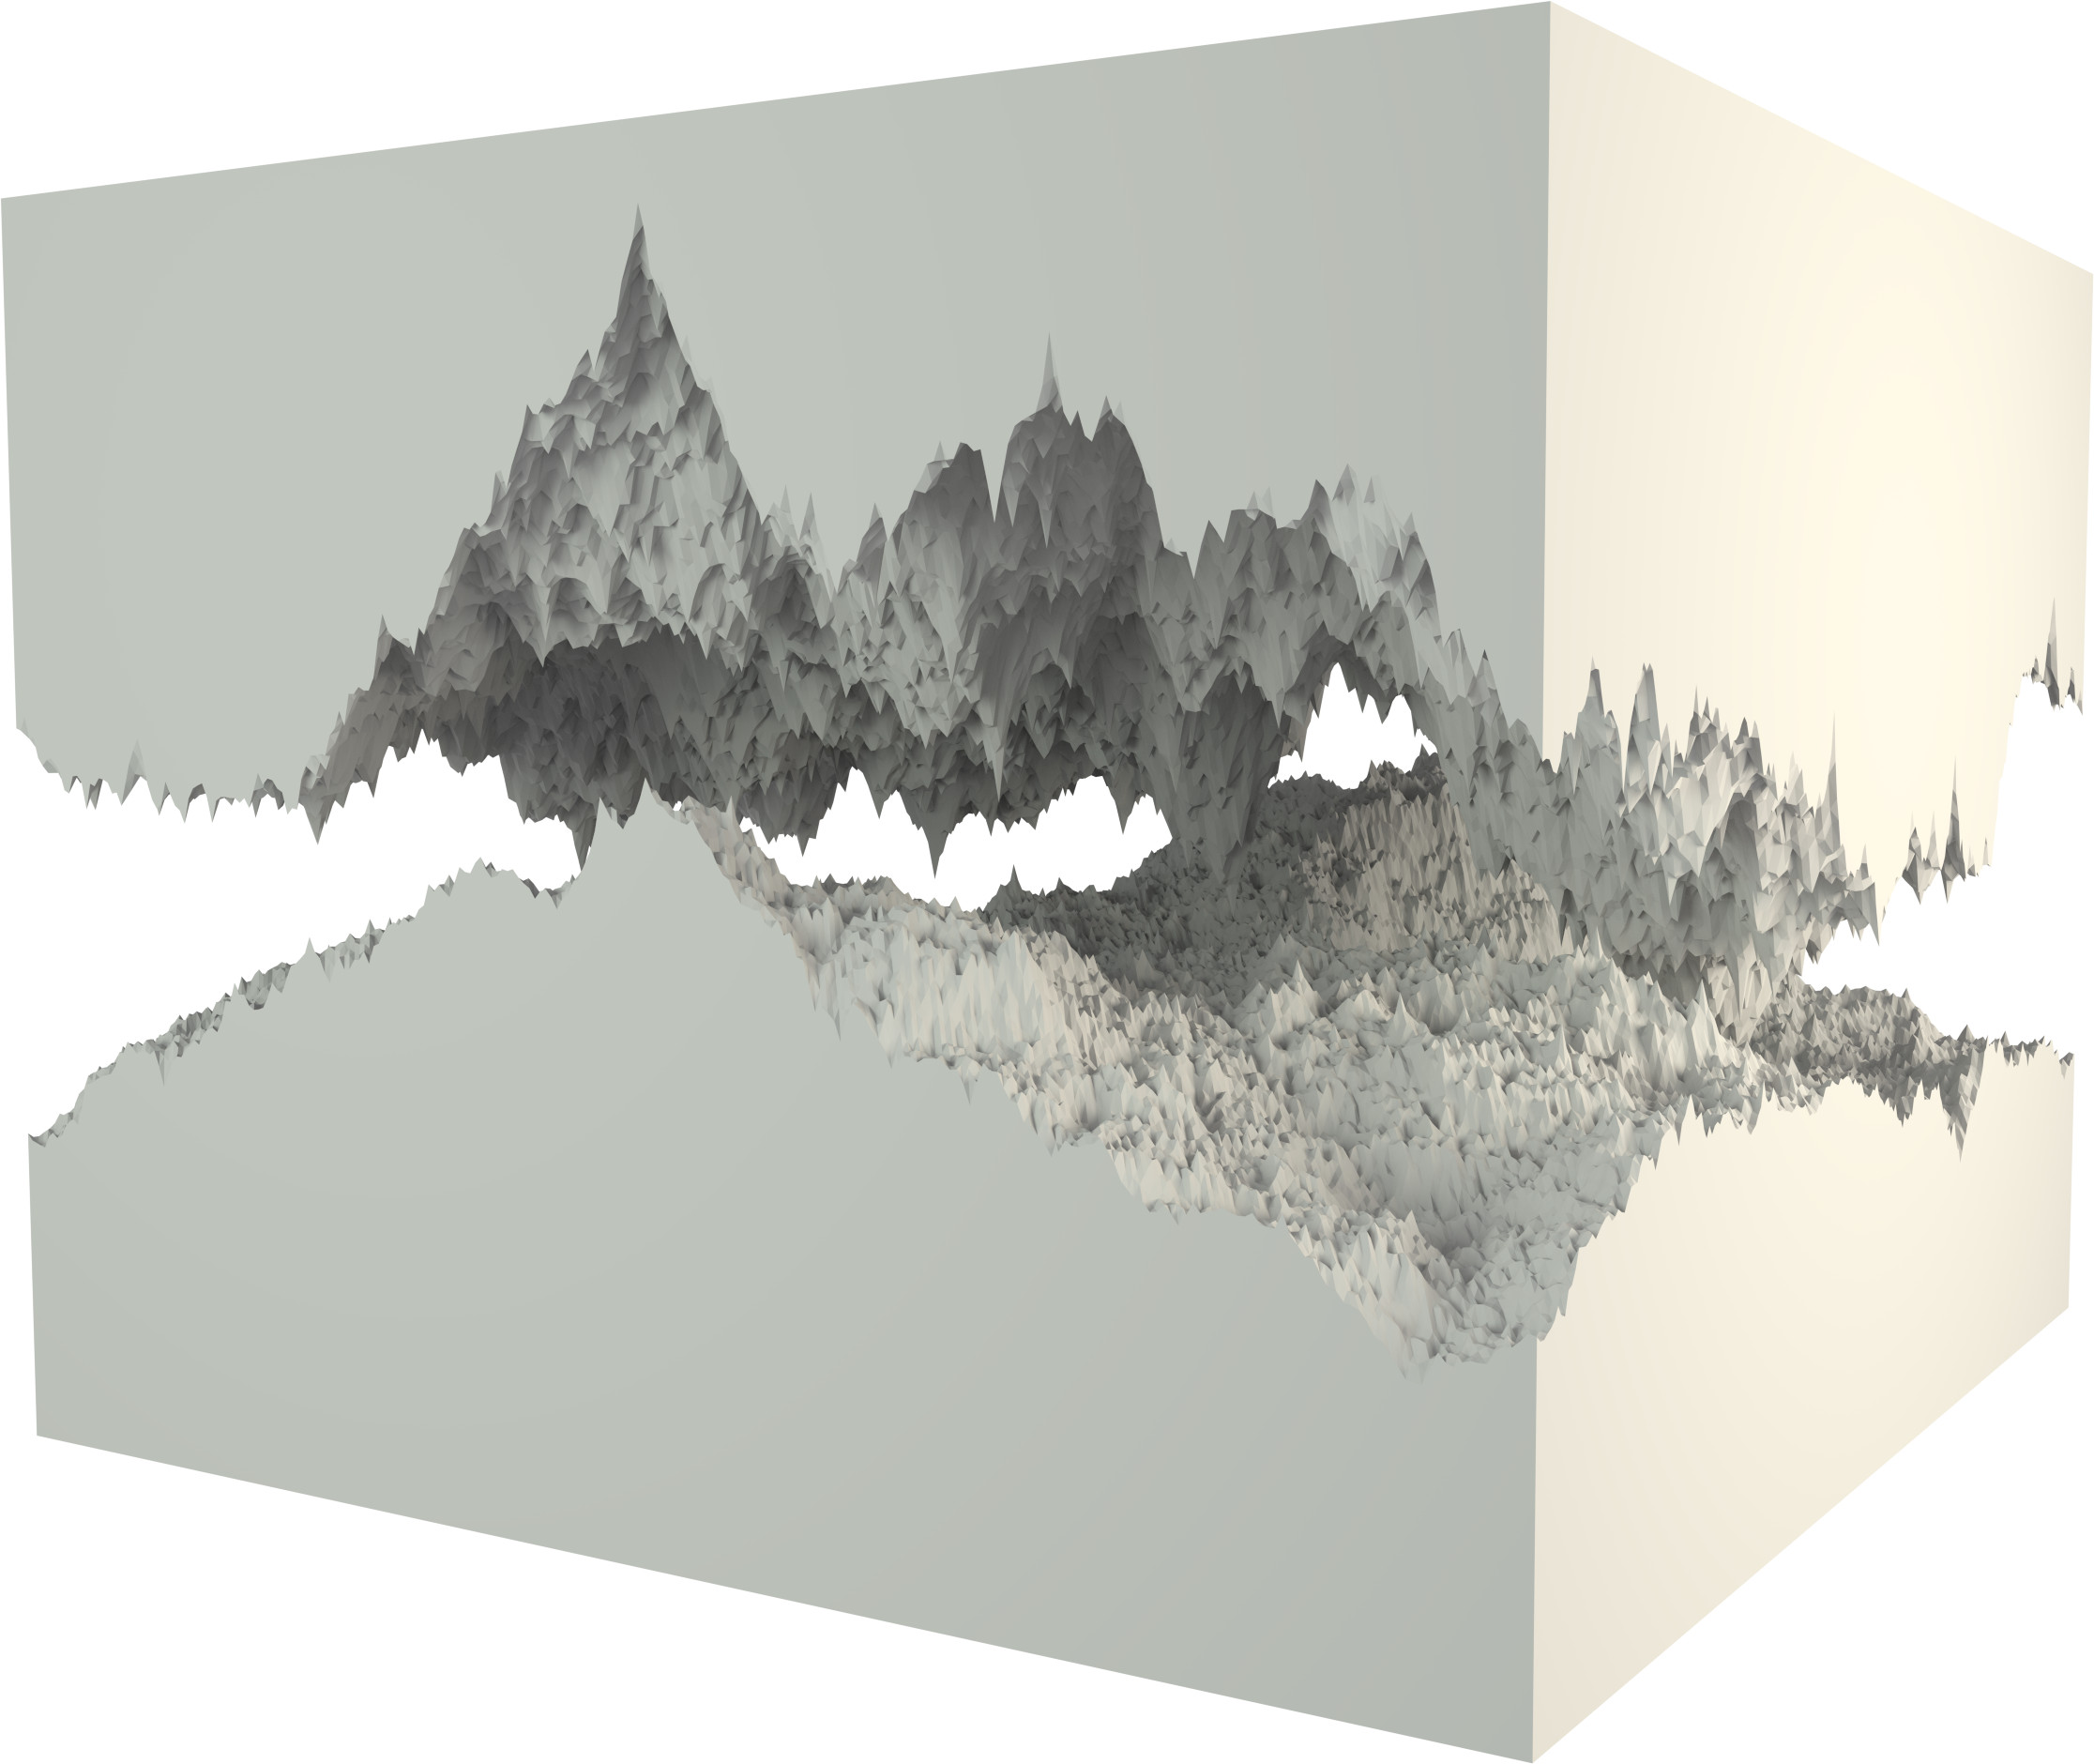
\includegraphics[width=\textwidth]{images/fracture/large_fracture05.jpg}%
    \caption{Caption}%
\end{figure}%

\chapter{Introduction}
We want to study the behaviour of water trapped in nanoscale pores and fractures in silica, so need a way to generate and characterize such structures. Like a lot of phenomena in nature, we can describe and generate fractures using the theory of fractals\cite{mandelbrot1983fractal}. 

\orangebox{
\begin{itemize}
    \item Define fractal
    \item Define/explain self-similarity and similar terms
\end{itemize}

}


To generate a fractal surface we will use fractional Brownian motion \hl{(fBm)}, introduced by Mandelbrot and van Ness in 1968\cite{mandelbrot1968fractional}. Fractional Brownian motion is a process which generates \hl{data} that \hl{is fractal}, in the sense that it is self-similar. The \hl{data} generated by this process can be characterized by a parameter denoted $H$, often called the Hurst exponent. $H$ is related to the \hl{autocorrelation (define?)} of a data set, and is always a number between 0 and 1. It is directly related to the fractal dimension $D$ via \hl{source?}
\begin{align*}
    D = d - H
\end{align*}

\hl{The Hurst exponent quantifies the relative tendency of a (time series) to either regress to the mean, or to cluster in a direction.} $H\in[0,0.5]$ indicates a \hl{time series} with long-term switching between high and low values in adjacent pairs, meaning that a single high value will probably be followed by a low value, and vice versa. $H\in[0.5,1.0]$ indicates a \hl{time series} with long-term positive autocorrelation, meaning both that a high value will probably be followed by another high value, and that the values a long time into the future will also tend to be \hl{high (increasing?)}.

Samples of \hl{fBm} with different Hurst parameters will differ in what can quantitatively be called the ``roughness'' or the ``randomness'' of the \hl{series}, as can be seen in \cref{fig:fBm_examples}.

in honor of both Harold Edwin Hurst and Ludwig Otto H\"older

The Hurst exponent and the use of it as a means of characterizing a \hl{dataset/timeseries?} was developed \hl{in the field of hydrology}, as seen in \cite{hurst1951longterm,hurst1965longterm}, where it was used to determine the optimal dam sizing for the Nile river's, by studying the large fluctuations in the flow rate of the river, which had been observed over a long time period\todo{rewrite this one-sentence paragraph}. It is denoted $H$ in honor of both Harold Hurst, who was the lead researcher in these studies, and in honor of Otto H\"older \hl{WHY H\"older?}.

\orangebox{
\begin{itemize}
    \item No true fractals in nature, since we need infinite resolution
    \item $H = $ Hausdorff dimension? index-$\alpha$?
    \item See \cite{mu1988steel} for ref. on fractal dimension of fractured steel surface
\end{itemize}

}

%
\begin{figure}[htpb]%
    \centering%
    \includesvg[width=0.7\textwidth, svgpath = ./images/Hurst/]{fbm_1d_examples_grid}%
    \caption{}%
    \label{fig:fBm_examples}%
\end{figure}%
\begin{figure}[htpb]%
    \centering%
    \includesvg[width=1.0\textwidth, svgpath = ./images/Hurst/]{fbm_1d_examples}%
    \caption{}%
%     \labedl{fig:fBm_examples01}%
\end{figure}%

% We will use fractional Brownian motion (fBm) to 
% We use fractional Brownian motion (fBm) to model fractures 

% We will use fractals both for describing, and for generating fractures.

% (Several methods of characterizing a fracture could be imagined (\hl{SOURCES, examples}), and we will use several of them.)        

% \hl{terrain == heightmap??, finn bra ord her}

\orangebox{
    \begin{itemize}
        \item Plot 1D DMA estimate vs. synthesized 1D fBm from FracLab. Difference between with and without new $f^*$.
        \item Plot 2D DMA estimate vs. synth. 2D fBm from FracLab? \hl{Does FracLab generated 2D?}
        \item Plot 2D DMA est. vs. input Hurst for diamond square. Compare with and without addition and PBC.
    \end{itemize}

}

\chapter{Fractals and fractures}

\todo{change wording? copied from Fractals...}
An \emph{affine transformation} transforms a point $\bvec x = (x_1, \dots, x_n)$ into new points $\bvec x' = (r_1x_1, \dots, r_n, x_n)$, where the scaling rations $r_1, \dots, r_n$ are \emph{not} all equal.

A bounded set $\mathcal{S}$ is \emph{self-affine} if $\mathcal{S}$ is the union of $N$ non-overlapping subsets $\mathcal{S}_1, \dots, \mathcal{S}_N$, each of which is congruent to the set $\bvec r(\mathcal{S})$ obtained from $\mathcal S$ by the affine transform defined by $\bvec r$. Here \emph{congruent} means that the set of points $\mathcal{S}$ is identical to the set of points $\bvec r(\mathcal{S})$ after possible translations and/or rotations of the set\cite{feder1988fractals}.

A set $\mathcal{S}$ is \emph{statistically self-affine} if $\mathcal{S}$ is the union of $N$ non-overlapping subsets each of which is scaled down by $\bvec r$ from the original, and is identical in all statistical respects to $\bvec r(\mathcal{S})$.

% \section{Surface area}
% \section{Distance to nearest atom}
\begin{itemize}
    \item Fractals
    \item Fractional Brownian Motion
    \item The Hurst Exponent
\end{itemize}
